\documentclass[micros_g1_main.tex]{subfiles}
\begin{document}

\section{}

Se realiz\'o un memory dump de la posici\'on A000 en adelante. El resultado obtenido se observa en la figura \ref{fig:memory-dump}.

\begin{figure}[ht]
	\centering
	\fbox{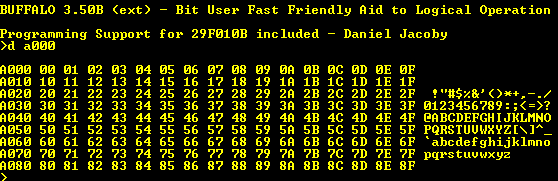
\includegraphics[width=0.8\textwidth]{images/micros-g1-ej2.png}}
	\caption{Memory dump de la posici\'on de memoria A000 en adelante}
	\label{fig:memory-dump}
\end{figure}

Estas posiciones se encuentran en una zona libre de la memoria, es decir que no corresponden a ninguna memoria f\'isica. Por lo tanto, lo que se obtiene en la terminal no puede corresponder realmente a un dato que se ley\'o. 

Se observa que la lectura obtenida coincide con la parte baja del n\'umero de posici\'on (la posici\'on A000 devuelve 00, la A001 devuelve 01, etc\'etera). Esto puede explicarse si se considera que el bus de datos se utiliza tambi\'en para transmitir la parte baja de la direcci\'on (el bus est\'a multiplexado). Cuando E cambia de 0 a 1, el bus pasa a baja impedancia, pero por las capacidades par\'asitas presentes en el microprocesador, como nadie fuerza un valor al bus, queda en el estado anterior. Dicho estado no es otra cosa que el byte menos significativo de la direcci\'on.

\end{document}
